
%(BEGIN_QUESTION)
% Copyright 2010, Tony R. Kuphaldt, released under the Creative Commons Attribution License (v 1.0)
% This means you may do almost anything with this work of mine, so long as you give me proper credit

Calculate the three distances ($x_1$, $x_2$, and $x_3$) in this radar level measurement application given times between echo pulses of 10.7 ns, 31.8 ns, and 80.5 ns, respectively:

$$\includegraphics[width=15.5cm]{i04622x01.eps}$$

$x_1$ = \underbar{\hskip 50pt}

\vskip 10pt

$x_2$ = \underbar{\hskip 50pt}

\vskip 10pt

$x_3$ = \underbar{\hskip 50pt}

\vskip 10pt

\underbar{file i04622}
%(END_QUESTION)





%(BEGIN_ANSWER)

$x_1$ = 1.27 m

\vskip 10pt

$x_2$ = 1.23 m

\vskip 10pt

$x_3$ = 1.82 m

%(END_ANSWER)





%(BEGIN_NOTES)


%INDEX% Measurement, interface level: radar

%(END_NOTES)


